\documentclass{boi2014-lt}

\usepackage{enumitem}
\usepackage{todonotes}

\renewcommand{\DayNum}{0}
\renewcommand{\TaskCode}{network}
\renewcommand{\TaskName}{Computer Network}

\begin{document}
    Vidurinės mokyklos kompiuterių klasėje $N$ kompiuterių yra kabeliais
    sujungti į bendrą tinklą. Kiekvienas kabelis jungia du skirtingus
    kompiuterius. Kai kurie kompiuteriai gali būti nesujungti kabeliu
    tiesiogiai, tačiau tarp bet kurių dviejų kompiuterių galima persiųsti
    pranešimą tiesiogiai arba per tarpinius kabeliais sujungtus kompiuterius.
    Pranešimai visada pasirenka trumpiausią kelią, t.y. pakeliui aplanko
    mažiausią galimą skaičių kompiuterių (neskaičiuojant pranešimą siunčiančio
    ir gaunančio kompiuterių).
    
    Adam ir Billy, kurie klasėje naudojasi skirtingais kompiuteriais $a$ ir $b$,
    norėtų rasti trumpiausią kelią tarp savo kompiuterių. Jie nežino, kaip
    išvedžioti kabeliai, bet gali siųsti pranešimus tarp kiekvienos
    kompiuterių poros ir suskaičiuoti, kiek tarpinių kompiuterių siunčiami
    pranešimai aplanko.
    
    Adam ir Billy nelabai gaudosi kompiuteriuose, tad prašo jūsų pagalbos, kad
    netektų siųsti per daug pranešimų.

    \Task
    Raskite trumpiausią kelią tarp kompiuterių $a$ ir $b$ siųsdami ne daugiau
    negu leistiną skaičių pranešimų.

    \Implementation
    Jums reikia realizuoti vieną procedūrą \method{findRoute(N, a, b)}, kurios argumentai yra:

    \begin{itemize}
        \item $N$ --- klasėje esančių kompiuterių skaičius
            (jie sunumeruoti nuo $1$ iki $N$)
        \item $a, b$ --- Adam ir Billy kompiuterių numeriai
            ($a \neq b$ ir $1 \le a, b \le N$)
    \end{itemize}

    Jūsų procedūra \method{findRoute} gali kviesti funkciją \method{ping(i, j)},
    kurios argumentai yra dviejų skirtingų kompiuterių numeriai
    ($i \neq j$ ir $1 \le i, j \le N$), o grąžinama reikšmė --- tarpinių
    kompiuterių skaičius pranešimui keliaujant iš kompiuterio $i$ į
    kompiuterį $j$.

    Jūsų procedūra \method{findRoute} turi nusakyti trumpiausią kelią, kurį
    nukeliaus pranešimas, išsiųstas iš kompiuterio $a$ į kompiuterį $b$. Tai
    turi būti atliekama pakartotinai kviečiant procedūrą \method{travelTo(k)} su
    vieninteliu argumentu --- kompiuterio, į kurį turi keliauti
    pranešimas kitu ėjimu ($1 \le k \le N$), numeriu. Pranešimas kelionę pradeda
    kompiuteryje $a$ ir, kai tik iškviečiama procedūra \method{travelTo(k)}, jis
    persikelia į kompiuterį $k$.

    Papildomai prie standartinių reikalavimų (laiko ir atminties ribojimai,
    jokių vykdymo klaidų), jūsų sprendimas turėtų tenkinti šiuos papildomus
    reikalavimus:

    \begin{itemize}
        \item procedūrai \method{findRoute} baigus darbą pranešimas turėtų būti
            kompiuteryje $b$,
        \item pranešimo kelyje visi gretimi kompiuteriai privalo būti tiesiogiai
            sujungti kabeliu,
        \item tai turi būti trumpiausias galimas kelias,
        \item funkcijos \method{ping} iškvietimų skaičius neturi viršyti $M$
            (žr. skyrių Vertinimas),
        \item funkcija \method{ping} ir procedūra \method{travelTo} privalo būti
            kviečiamos tik su leistinomis argumentų reikšmėmis.
    \end{itemize}

    \Example
    Tarkime, kad duotas kompiuterių tinklas atrodo taip, kaip pavaizduotas
    diagromoje žemiau (taškai žymi kompiuterius, o atkarpos --- kabelius). Iš
    viso tinkle yra $N = 4$ kompiuteriai, o Adam ir Billy naudojasi
    kompiuteriais $a = 1$ ir $b = 4$.

    \begin{wrapfigure}[1]{r}{5cm}
        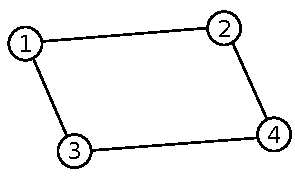
\includegraphics{network-example}
    \end{wrapfigure}

    Pirmiausiai bus iškviesta procedūra
    \begin{figure}[H]
        \centering
        \method{findRoute(4, 1, 4)}.
    \end{figure}

    Vienas galimas jos elgesys galėtų būti toks::

    \begin{figure}[H]
        \centering
        kviečiama funkcija \method{ping(1, 4)}, kuri grąžina $1$, \\
        kviečiama funkcija \method{ping(1, 2)}, kuri grąžina $0$, \\
        kviečiama funkcija \method{ping(2, 4)}, kuri grąžina $0$.
    \end{figure}

    Šios informacijos pakanka, kad rastume trumpiausią kelią $1 \to 2 \to 4$ iš
    kompiuterio $1$ į kompiuterį $4$. Rastas kelias turėtų būti įvardintas tokiu
    būdu:

    \begin{figure}[H]
        \centering
        kviečiama procedūra \method{travelTo(2)}, \\
        kviečiama procedūra \method{travelTo(4)}, \\
        procedūra \method{findRoute} baigia darbą.
    \end{figure}

    \Scoring
    Visose užduočių grupėse galioja apribojimas $2 \le N \le 1000$.

    \begin{description}
        \item[Subtask 1 (25 points):] tarp bet kurių dviejų kompiuterių yra
            lygiai vienas trumpiausias kelias; $M$ negali viršyti $2N$.
        \item[Subtask 2 (25 points):] $M$ negali viršyti $N^2$.
        \item[Subtask 3 (25 points):] $M$ negali viršyti $4N$.
        \item[Subtask 4 (25 points):] $M$ negali viršyti $2N$.
    \end{description}

    \Constraints
    \begin{description}
        \item[Time limit:] 1 s.
        \item[Memory limit:] 64 MB.
    \end{description}

    \Experimentation
    Jūsų kompiuteryje esantis pavyzdinis vertintojas nuskaitys duomenis iš
    standartinės įvesties. Pirmoje eilutėje turėtų būti keturi sveikieji
    skaičiai $N, a, b, M$. Kitose $N$ eilučių turėtų būti po $N$ sveikųjų
    skaičių, apibūdinančių kabelių išdėstymą:
    $j$--asis skaičius $i$--ojoje eilutėje ($i \neq j$) žymi tarpinių
    kompiuterių, kurį aplankys pranešimas keliaudamas iš kompiuterio $i$ į
    kompiuterį $j$, skaičių. Jeigu $i = j$, gali būti nurodytos bet kokios
    reikšmės.

    Žemiau pateikta įvestis nusako anksčiau pateiktą pavyzdį, kai iškvietimų
    skaičius $M$ apribotas iki $100$:

    \begin{center}
        \begin{tabular}{p{4cm}}
            {\tt
                4 1 4 100 \newline
                0 0 0 1 \newline
                0 0 1 0 \newline
                0 1 0 0 \newline
                1 0 0 0
            }
        \end{tabular}
    \end{center}

\end{document}

